%----------------------------------------------------------------------------- %%
\section{Descheduler Design}
\label{bab:3}
%----------------------------------------------------------------------------- %%

\begin{figure*}[t!]
	\centering
	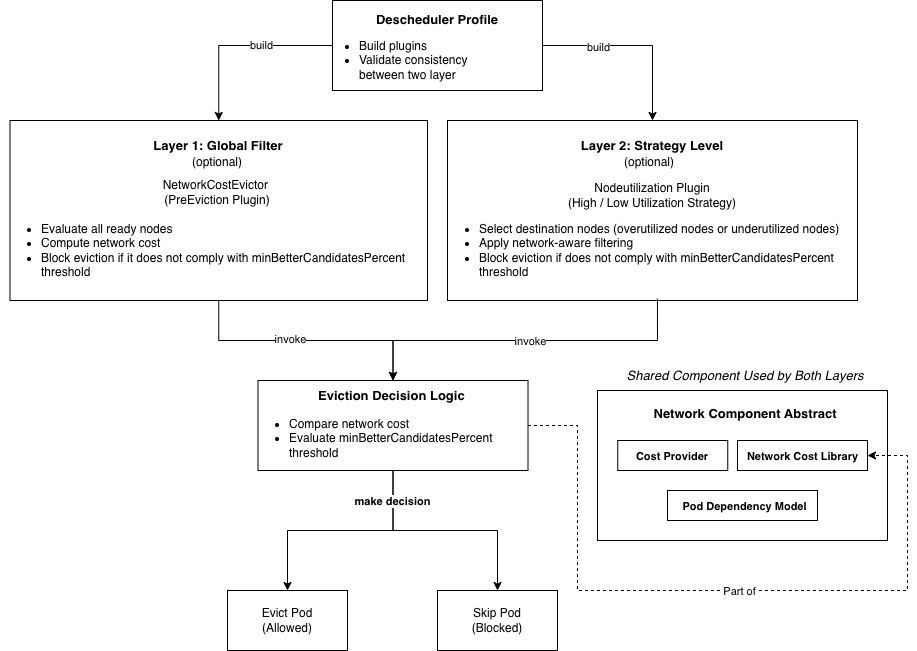
\includegraphics[width=0.95\textwidth]{assets/pics/network-aware/sysarc-diagram.png}
	\caption{Network-Aware plugin architecture design.}
	\label{fig:netaware_arcdesign}
\end{figure*}

\subsection{Architecture Overview}
The Network-Aware Evictor is developed as a Kubernetes Descheduler extension designed to safeguard network locality during cluster consolidation. The plugin incorporates topology-based and latency-based cost models to prevent the descheduler from moving dependent microservices to distant or degraded nodes. 

As illustrated in Figure \ref{fig:netaware_arcdesign}, the system utilizes a two-layer plugin architecture that abstracts the Network Cost Model into a Cost Provider. The primary layer is a dedicated \texttt{PreEvictionFilter} extension integrated into the standard Kubernetes Descheduler framework. In this framework, the filter is executed immediately before an eviction request is submitted. Pre-eviction filters can be chained; therefore, a candidate Pod must pass the network-aware filter before the descheduler performs the eviction. By executing as a pre-eviction safety gate, the plugin intercepts standard strategy-driven eviction decisions before they are finalized. 

The plugin can be deployed as a global \texttt{PreEvictionFilter} to prevent evictions that would increase the total network cost across all candidate nodes. Alternatively, it can be incorporated directly into node utilization strategies, offering a more targeted filtering mechanism by only analyzing the destination nodes selected by the strategy. The Cost Provider abstraction cleanly separates this core filtering logic from the underlying network metrics, allowing the system to dynamically swap between different cost calculation strategies without altering the primary descheduling pipeline.


\subsection{Network Cost Model}
To accommodate various deployment situations, the Network Cost Model supports two methodologies. The topology-based cost model calculates the network cost based on the node locality information (zone and region). It assigns specified costs based on relative position, assuming that latency rises with logical distance (e.g., same-zone=1, same-region=5, cross-region=10). This model is lightweight and requires no external monitoring. Alternatively, the latency-based cost model computes the network cost according to observed node-to-node communication performance, adapting to dynamic cluster conditions. This requires integration with a Prometheus-based monitoring infrastructure (such as Goldpinger) to scrape real-time latency measurements between nodes. Both layers of the plugin must use consistent configurations to prevent conflicting eviction decisions.

\subsection{Eviction Decision Workflow}
The network-aware eviction workflow operates after the built-in \texttt{DefaultEvictor} confirms basic scheduling constraints. The process operates as a sequence of decision gates. First, the plugin inspects the candidate pod to determine if a network dependency label (e.g., \texttt{network-group}) exists. If no defined dependencies exist, the plugin immediately allows the eviction.

If a dependency label is found, the algorithm identifies all related dependency pods using Kubernetes owner references and label matching. It then calculates the baseline network cost by computing the communication overhead between the candidate pod's current node and all nodes hosting its dependencies. Next, it retrieves potential candidate destination nodes and computes the hypothetical network cost that would occur if the pod were rescheduled to that location. The pairwise communication cost for both the current placement and all candidate nodes is computed using the procedure detailed in Algorithm 1.

\vspace{0.5em}
\noindent\rule{\linewidth}{0.4pt}
\textbf{Algorithm 1:} Compute Placement Cost algorithm
\vspace{-0.5em}

\noindent\rule{\linewidth}{0.4pt}
\textbf{Input:} \textit{candidateNode, D, nodesMap, costProvider} \\
\textbf{Output:} \textit{totalCost}
\vspace{-0.5em}
\begin{algorithmic}[1]
\STATE \textit{totalCost} $\leftarrow 0$
\FOR{\textbf{each} pod $d \in D$}
    \STATE \textit{depNode} $\leftarrow$ \textit{nodesMap}[$d$.\textit{nodeName}]
    \IF{\textit{depNode} \textbf{not found}}
        \STATE \textbf{continue}
    \ENDIF
    \STATE \textit{totalCost} $\leftarrow$ \textit{totalCost} $+$ 
    \STATE \hspace{1em} \textit{Cost}(\textit{candidateNode}, \textit{depNode})
\ENDFOR
\RETURN \textit{totalCost}
\end{algorithmic}
\vspace{-0.5em}
\noindent\rule{\linewidth}{0.4pt}
\vspace{0.5em}

An eviction is permitted only if the number of candidate destination nodes satisfying the condition (resulting network cost is less than or equal to the baseline cost) exceeds the minimum threshold percentage of the total candidates (defaulting to 50\%). This threshold-based mechanism balances workload redistribution with communication efficiency, increasing the likelihood that the scheduler will subsequently place the evicted pod onto a node that preserves network locality.

\subsection{Plugin Configuration}
The Network-Aware policy is configured through two layers. The global \texttt{NetworkCostEvictor} configures parameters for dependency identification, minimum threshold percentage, pods ownership filtering, and optional latency-based cost evaluation. The second configuration extends existing node utilization strategies with identical network-aware blocks, ensuring consistent filtering behavior but potentially applying different levels of strictness via the threshold parameter. The full YAML configuration structures for both the global L1 filter and the strategy-embedded L2 filter are provided in Appendix \ref{appendix:netaware_configL1} and Appendix \ref{appendix:netaware_configL2}, respectively.
